%----------------------------------------------------------------------------------------
%	PACKAGES & THEMES
%----------------------------------------------------------------------------------------

\documentclass[8pt]{beamer}

\usepackage{etex}
\mode<presentation> {

\usetheme{Vilanova}
}



\usepackage[english]{babel}
\usepackage[utf8]{inputenc}
\usepackage{array}
\usepackage{chronology}
\let\CHRONOLOGY\chronology
\let\endCHRONOLOGY\endchronology
\def\chronology{\shorthandoff{;}\CHRONOLOGY}
\def\endchronology{\endCHRONOLOGY\shorthandon{;}}
\usepackage{pstricks}
\usepackage{graphicx}
\usepackage{booktabs}
\usepackage{amsmath,amssymb,amsthm}
\usepackage{xcolor}
\usepackage{textpos}
\usepackage{tikz}
\usepackage{xmpincl}
\usetikzlibrary{arrows}
\usepackage{pifont}

\usepackage{listings,color}

\definecolor{listcomment}{rgb}{0.0,0.5,0.0}
\definecolor{listkeyword}{rgb}{0.0,0.0,0.5}
\definecolor{listnumbers}{gray}{0.65}
\definecolor{listlightgray}{gray}{0.955}
\definecolor{listwhite}{gray}{1.0}


%% \setbeamertemplate{background canvas}{\includegraphics
%%    [width=\paperwidth,height=\paperheight]{./images/title.pdf}}

\AtBeginSection[]
{
\addtocounter{framenumber}{-1}
\begin{frame}
\frametitle{Sommaire}
\tableofcontents[currentsection]
\end{frame}}

%----------------------------------------------------------------------------------------
%	PAGE TITRE
%----------------------------------------------------------------------------------------
\title{Orfeo ToolBox users meeting and hackfest 2015}
\includexmp{images/cc}
\subtitle{Third parties policy and SuperBuild}
\author{OTB development team}% date and event here
\date{3 - 5 june 2015, Toulouse}

\pgfdeclareimage[height=96mm,width=128mm]{background}{images/fondsClairSansLogo}
\pgfdeclareimage[height=0.2cm]{cc}{images/CC-licence.png}
\setbeamertemplate{background}{\pgfuseimage{background}}
\pgfdeclareimage[height=0.6cm]{logoIncrust}{images/logoIncrust}
\logo{
\begin{tabular}{p{0.22\textwidth}p{0.58\textwidth}p{0.1\textwidth}p{0.1\textwidth}}
\href{http://creativecommons.org/licenses/by-sa/3.0/}{\pgfuseimage{cc}}
& \vspace{-0.03\textwidth} \scriptsize{} % date and event here
&  & \href{http://www.orfeo-toolbox.org}{\pgfuseimage{logoIncrust}}\\
\end{tabular}
}

\begin{document}
\begin{frame}
\titlepage
\end{frame}

\begin{frame}
\frametitle{Third parties in OTB}

\begin{itemize}
\item Reduced number of third parties, goodbye to Edison, ConfigFile, Expat, msinttypes
\item Reduced dependency contamination with optional third parties
\end{itemize}

\begin{center}
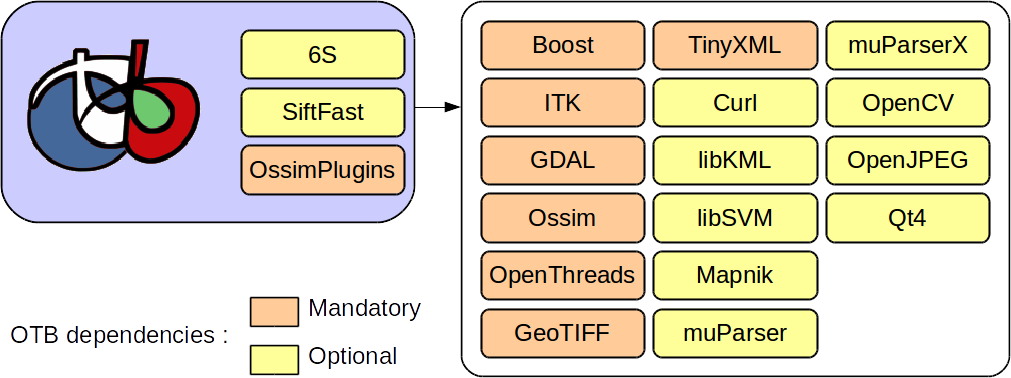
\includegraphics[height=4cm]{images/otb_3rd_parties}
\end{center}

\end{frame}

\begin{frame}
\frametitle{Third parties integration}

\begin{itemize}
\item Almost all third parties source code is removed from OTB (except with 6S, Siftfast and OssimPlugins)
\item "External" dependencies have to be installed by the user
\item One module for each third party, containing a CMake call to \texttt{find\_package(\ldots)}
\item Located in source directory \emph{OTB/Modules/ThirdParty}
\item Optional third parties enabled / disabled using specific CMake options : OTB\_USE\_ \ldots
\end{itemize}



\end{frame}

\begin{frame}
\frametitle{SuperBuild : why ?}

\begin{itemize}
\item Reduce the effort to prepare an environment ready for OTB compilation
\begin{itemize}
\item Before OTB 5.0 , this was partially done using internal third-parties
\item External dependencies imply different versions and compilation settings depending on the user platform
\item Lots of issues coming from incompatible versions or library setup
\end{itemize}
\item Need to identify a set of third parties (with their version and compilation options) 
that is known to work well with OTB on all supported platforms
\item Final purpose : be able to build OTB on any platform with a compiler and CMake (\textgreater = 2.8.11)
\end{itemize}

\end{frame}

\begin{frame}
\frametitle{SuperBuild : how ?}

\begin{itemize}
\item At compilation time, CMake will download, patch, configure, build and 
install third parties as \emph{external projects} (for details, check CMake 
\href{http://www.cmake.org/cmake/help/v3.2/module/ExternalProject.html}{ExternalProject})
\item Choice between system library and SuperBuild library
\item Each external project can declare a set of dependencies
\end{itemize}

\begin{center}
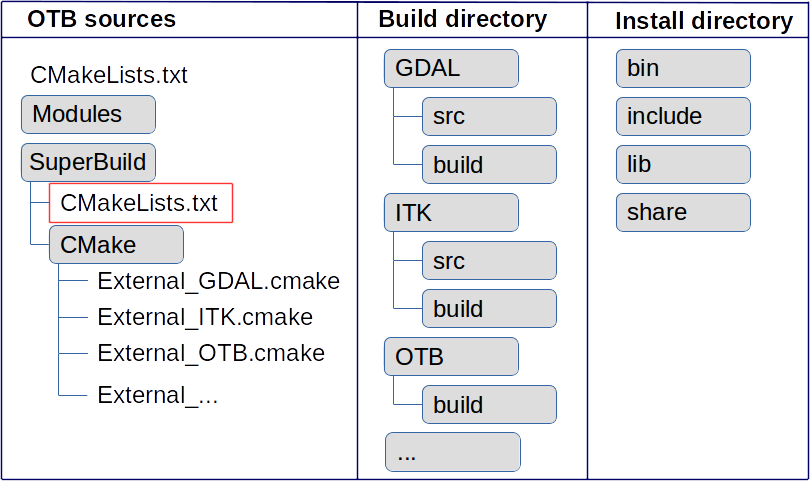
\includegraphics[height=5cm]{images/otb_superbuild_archi}
\end{center}

\end{frame}

\begin{frame}
\frametitle{SuperBuild : settings}

\begin{itemize}
\item \texttt{CMAKE\_INSTALL\_PREFIX} : should be set by the user as OTB and the dependencies 
built by SuperBuild will always be installed there (even whitout calling target "install")  
\item \texttt{OTB\_USE\_\ldots} : the activation options of OTB third parties are also available 
in SuperBuild. Depending on their value, they will trigger the activation of the 
corresponding dependencies.
\item \texttt{USE\_SYSTEM\_\ldots} : when a third party is needed, user may choose to use a 
version already installed on the system, or use the SuperBuild version.
\item \texttt{DOWNLOAD\_LOCATION} : directory used to download source archives. When archives 
are already present, no download is performed. An all-in-one archive is provided 
on OTB website for an offline compilation. Users should uncompress this archive 
and set this variable in order to use the 'offline' mode.
\end{itemize}

\end{frame}

\begin{frame}
\frametitle{SuperBuild : status}

\begin{center}
\begin{tabular}{|c|@{}c@{}|@{}c@{}|@{}c@{}||c|@{}c@{}|@{}c@{}|@{}c@{}|}
\hline
Third Party  & \multicolumn{3}{c||}{Support :} & Third Party  & \multicolumn{3}{c|}{Support :}\\
(version) & Linux & OSX & Win32 & (version) & Linux & OSX & Win32 \\
\hline
Boost (1.50.0) & x & x & x & OpenCV (2.4.10) & x & x & x\\
\hline
Curl (7.40.0) & & & x & OpenJPEG (2.1.0) & x & x & x\\
\hline
Expat (2.1.0) & x & x & x & OpenThreads (3.2.0) & x & x & x\\
\hline
FFTW (3.3.4) & x & x & x & Ossim (r23092) & x & x & x\\
\hline
GDAL (1.11.2) & x & x & x & PCRE (8.36) & & &\\
\hline
GEOS (3.4.2) & x & x & x & PNG (1.6.16) &  &  & x\\
\hline
GeoTIFF (1.4.0) & x & x & x & Proj4 (4.8.0) & x & x & x\\
\hline
ITK (4.7.1) & x & x & x & Qt4 (4.8.6) & & & x\\
\hline
Jpeg (9a) & x & x & x & SQLite (3.8.8.1) & x & x & x\\
\hline
libKML (1.3.0)\footnote{r863} & x & x & x & SWIG (3.0.5) & & & x\\
\hline
libSVM (3.20) & x & x & x & TIFF (4.0.3) & x & x & x\\
\hline
muParser (2.2.3) & x & x & x & TinyXML (2.6.2) & x & x & x\\
\hline
muParserX (3.0.5) & x & x & x & Zlib (1.2.8) & x & & x\\
\hline

\end{tabular}
\end{center}


\end{frame}


\end{document}
